% !TEX root = ../main.tex

\clearpage
% Source PDF page 45.
\section{第十章\quad 国际奶蛙传播人士}

在本章，我们将会了解一些致力于在国际平台传播奶蛙文化的人士和大学，或者本身被冠以奶之名的人士。

\textbf{【免责声明】}本章信息来源均来自于国内网络平台及聊天平台的流传图，渠道合法合规。请不要为了一睹国际奶蛙传播人士的风采而擅自使用违规工具进行违法网络活动。\textbf{若读者明知故犯，因此被抓获受到法律处罚，本书不承担包括但不限于诱导、教唆犯罪等相关法律责任。}~(见\figref{fig:10-1})

% !TEX root = ../../main.tex
\begin{figure}[H]
  \centering
  
\includegraphics[width=104.48bp,height=0.76\textheight,keepaspectratio]{figures/chapter10/figure10_1.pdf}
  \renewcommand{\thefigure}{10.1}
  \caption{奶察在看着你...}
  \label{fig:10-1}
\end{figure}


\subsubsection{（1）灰}

% !TEX root = ../../main.tex
\begin{figure}[H]
  \centering
  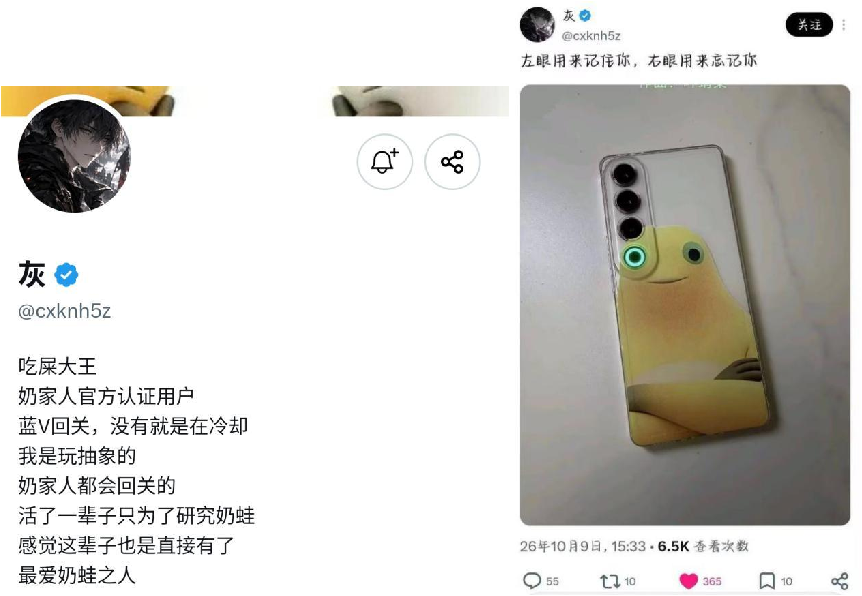
\includegraphics[width=351.83bp,height=0.76\textheight,keepaspectratio]{figures/chapter10/figure10_2.pdf}
  \renewcommand{\thefigure}{10.2}
  \caption{灰的 X（原推特）账号主页和被转到国内平台的相关推文}
  \label{fig:10-2}
\end{figure}


灰，奶国公民编号 000001，是一名奶蛙抽象大师。~(见\figref{fig:10-2})

他在 X 上高频率发送高质量 AI 奶蛙图文，并且自发为奶民提供奶国公民证编号（虽然概率很小啊，也可能是抽象的帽子叔叔利用 X 的关注可追溯性钓鱼）。其制作的部分图片或唯美（如一顿简单典雅的奶早餐、奶龙独自在美景中荡秋千）、

\clearpage
% Source PDF page 46.
\noindent 或科学（如《远古奶蛙灭绝事件研究：最后 24 小时》、《远古巨型奶蛙化石的发现及其演化意义》、《史前洞穴岩画中的奶蛙形象及其与早期人类的共存证据研究》等）。这些极具创造力的图片无疑为奶蛙的国内循环传播及对国外输出起到了极为重要的作用。~(见\figref{fig:10-3}, \figref{fig:10-4})

% !TEX root = ../../main.tex
\begin{figure}[H]
  \centering
  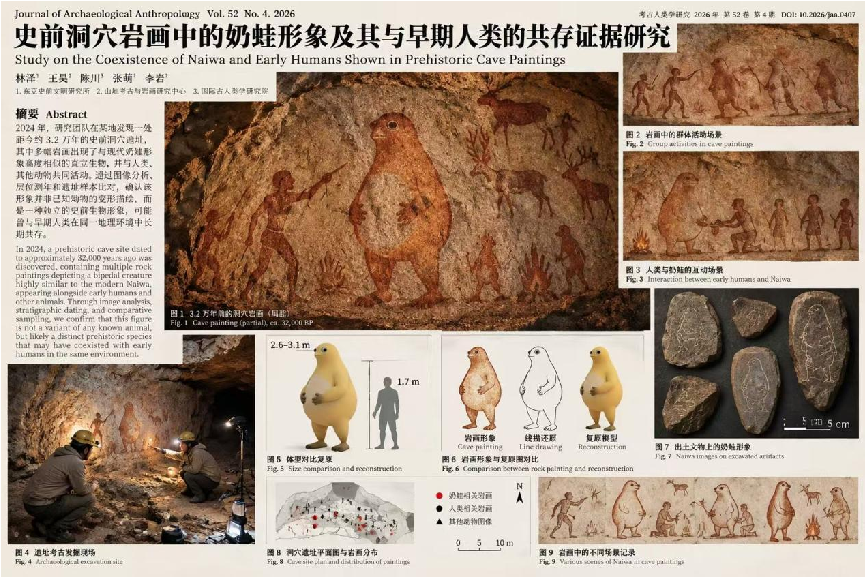
\includegraphics[width=353.36bp,height=0.76\textheight,keepaspectratio]{figures/chapter10/figure10_3.pdf}
  \renewcommand{\thefigure}{10.3}
  \caption{灰制作的一张奶蛙伪科学图解}
  \label{fig:10-3}
\end{figure}


% !TEX root = ../../main.tex
\begin{figure}[H]
  \centering
  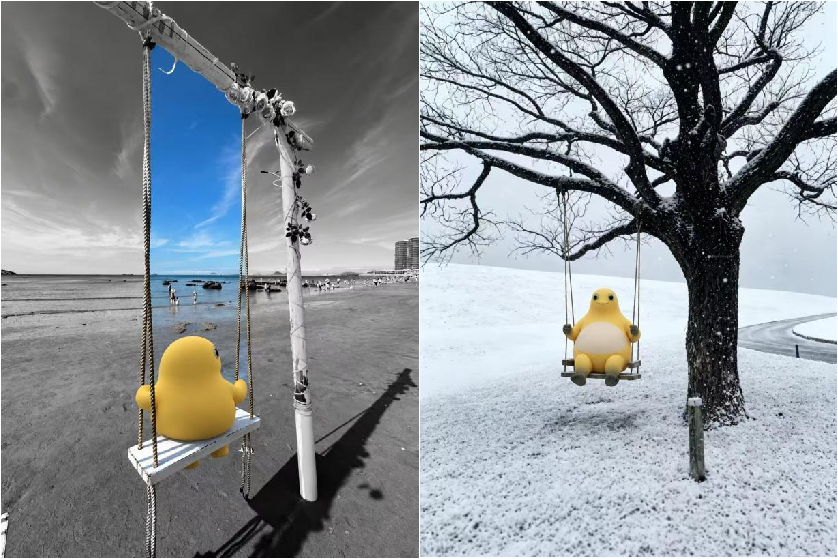
\includegraphics[width=342.04bp,height=0.76\textheight,keepaspectratio]{figures/chapter10/figure10_4.pdf}
  \renewcommand{\thefigure}{10.4}
  \caption{灰制作的两张极有意境的奶蛙秋千图}
  \label{fig:10-4}
\end{figure}


\subsubsection{（2）唐纳德·特朗普}

川宝，美国第 45、第 47 任美国总统，因为其金色的头发、极具张力的手风琴手势和捉摸不透的行政风格，被国内称别名为“奶龙”（被冠以奶之名の男）。~(见\figref{fig:10-5})

\clearpage
% Source PDF page 47.
% !TEX root = ../../main.tex
\begin{figure}[H]
  \centering
  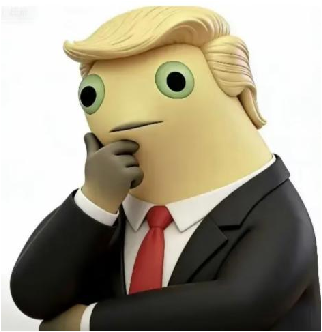
\includegraphics[width=131.41bp,height=0.76\textheight,keepaspectratio]{figures/chapter10/figure10_5.pdf}
  \renewcommand{\thefigure}{10.5}
  \caption{特朗普形象的奶蛙}
  \label{fig:10-5}
\end{figure}


\subsubsection{（3）埃隆·马斯克}

可能是因为 X 对用户账号的误封过于离谱，名字里又正好带个“隆”字，马斯克和奶家不知怎么地就莫名其妙地扯上了关系，变成了“奶隆”。~(见\figref{fig:10-6})

% !TEX root = ../../main.tex
\begin{figure}[H]
  \centering
  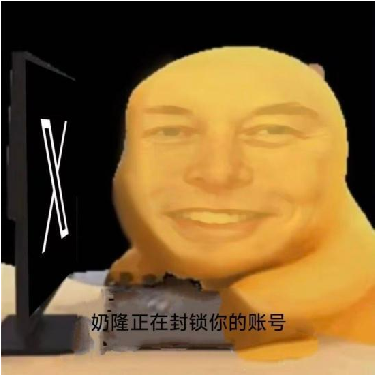
\includegraphics[width=111bp,height=0.76\textheight,keepaspectratio]{figures/chapter10/figure10_6.pdf}
  \renewcommand{\thefigure}{10.6}
  \caption{奶隆正在对 X 用户封号中}
  \label{fig:10-6}
\end{figure}


\subsubsection{（4）将军}

黑衣背头，捧腹大笑，这就是奶化二创里的“将军”。~(见\figref{fig:10-7})

% !TEX root = ../../main.tex
\begin{figure}[H]
  \centering
  
\includegraphics[width=68bp]{figures/chapter10/figure10_7.png}
  \renewcommand{\thefigure}{10.7}
  \caption{捧腹大笑的将军（二创）}
  \label{fig:10-7}
\end{figure}


\subsubsection[（5）密歇根大学]{（5）密歇根大学~(见\figref{fig:10-8})}

% !TEX root = ../../main.tex
\begin{figure}[H]
  \centering
  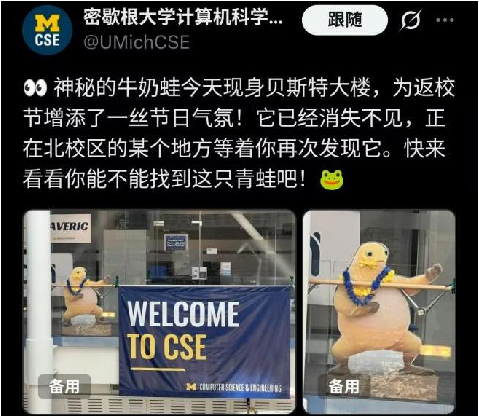
\includegraphics[width=154.87bp,height=0.76\textheight,keepaspectratio]{figures/chapter10/figure10_8.pdf}
  \renewcommand{\thefigure}{10.8}
  \caption{威斯康星大学麦迪逊分校的奶蛙形象}
  \label{fig:10-8}
\end{figure}


\clearpage
% Source PDF page 48.
\subsubsection[（6）威斯康星大学]{（6）威斯康星大学~(见\figref{fig:10-9})}

% !TEX root = ../../main.tex
\begin{figure}[H]
  \centering
  
\includegraphics[width=310.01bp,height=0.76\textheight,keepaspectratio]{figures/chapter10/figure10_9.pdf}
  \renewcommand{\thefigure}{10.9}
  \caption{纽约大学校徽（左）和身穿紫衣的 NYU 奶蛙立牌（右）}
  \label{fig:10-9}
\end{figure}


\subsubsection[（7）纽约大学]{（7）纽约大学~(见\figref{fig:10-10})}

% !TEX root = ../../main.tex
\begin{figure}[H]
  \centering
  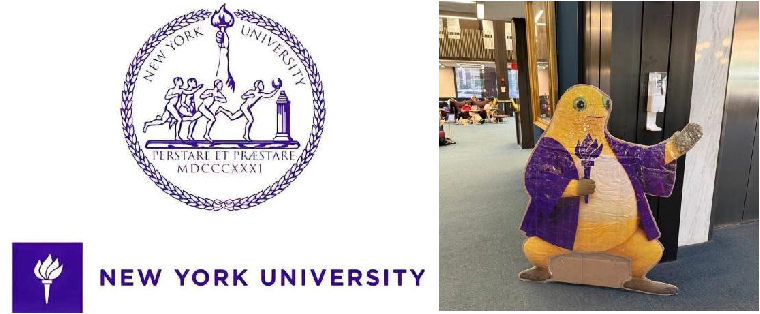
\includegraphics[width=188.43bp,height=0.76\textheight,keepaspectratio]{figures/chapter10/figure10_10.pdf}
  \renewcommand{\thefigure}{10.10}
  \caption{贴在柱子上的 UoA 奶蛙宣传单}
  \label{fig:10-10}
\end{figure}


\subsubsection[（8）奥克兰大学]{（8）奥克兰大学~(见\figref{fig:10-11})}

% !TEX root = ../../main.tex
\begin{figure}[H]
  \centering
  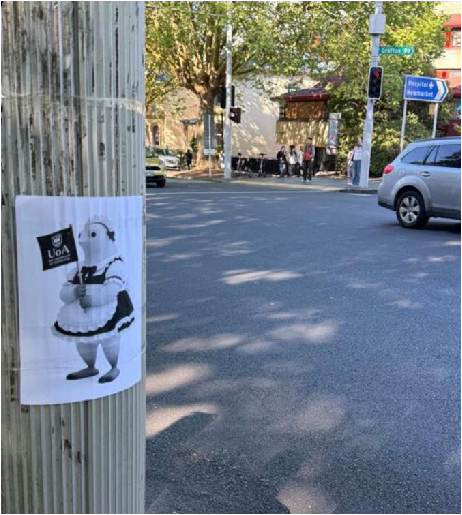
\includegraphics[width=188.43bp,height=0.76\textheight,keepaspectratio]{figures/chapter10/figure10_11.pdf}
  \renewcommand{\thefigure}{10.11}
  \caption{贴在柱子上的 UoA 奶蛙宣传单}
  \label{fig:10-11}
\end{figure}

